\subsection{Muon system {\it Keith, Yuri, Stepan, Larry}}

\label{sec:muon}


Searching for the A$^\prime$ in its di-muon decay mode has the advantage of having greatly reduced electromagnetic backgrounds for triggering.  The only physics background will arise from photoproduction of $\pi^+$ and $\pi^-$ pairs in the target, which aren�t fully absorbed in the ECal or absorber. The muon detector will be about 1 meter long and will consist of layers of scintillator hodoscopes sandwiched between iron absorbers. The number of layers and the thickness of absorbers is defined by the $\pi/\mu$ rejection factor. Detector was optimized using the GEANT-3 model of ECal, continued with layers of iron and scintillators. Muons in the momentum range from $1$ GeV to $4$ GeV has been studied, see \cite{HPS_PROP} for details.

In Figure \ref{fig:pmrej}, the rejection factor for charged pions is presented. As can be seen from the figure, for particles from $1$ GeV to $4$ GeV, the optimal thickness of the iron absorber for pion rejection is $\sim 75$ cm (after ECal, a $16$ cm of lead-tungstate). In the efficiency calculation for low energy particles ($< 1.7$ GeV) detection in in all four layers of scintillator hodoscopes were not considered. Depending on the momentum, particles were not traced behind the third, fourth or fifth absorber.  

\begin{figure*}[!ht]
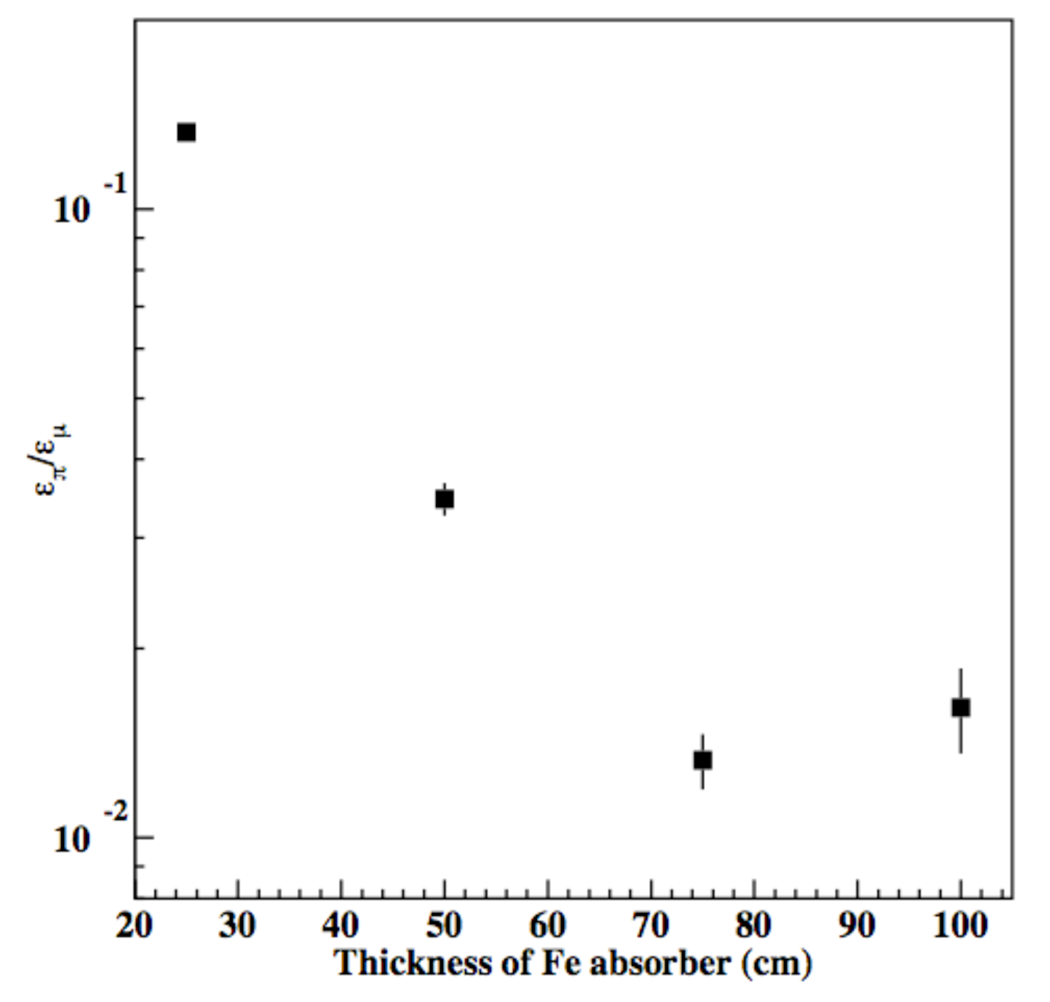
\includegraphics[scale=0.8]{muon/pmrej.pdf}
\caption{\small{Pion-muon rejection factor as a function of the iron absorber thickness.}}\label{fig:pmrej}
\end{figure*}


\subsubsection{Detector concept}

Based on simulations, a muon detector composed of a four iron absorbers (total length of $30+15+15+15=75$ cm) and four double-layer scintillator planes, positioned after each absorber layer is proposed. The muon detector will be mounted behind the ECal, see Figure 4.5.2.1. The pion rejection ($\pi/\mu$) of the proposed system as a function of particle momentum is shown in Figure \ref{fig:pmrejp}. For the determination of particle detection efficiencies, only signals in the first three layers of the hodoscope were used for momenta $< 1.7$ GeV/c. In the full momentum range from $1$ to $4$ GeV/c, $\pi/\mu$ varies from $10^{-2}$ to $2\times 10^{-2}$ and therefore the pion pair suppression factor of the system will be $< 4\times10^{-4}$. Similar to the Ecal, the muon detector will consist of two halves, one above and one below the beam. The vertical gap between the first hodoscope layers of the two halves is about 3 cm. The cross section of each half of the first hodoscope is $63\times 39$ cm$^2$. Each half of the last hodoscope layer is $74\times 46$ cm$^2$.  

\begin{figure*}[!ht]
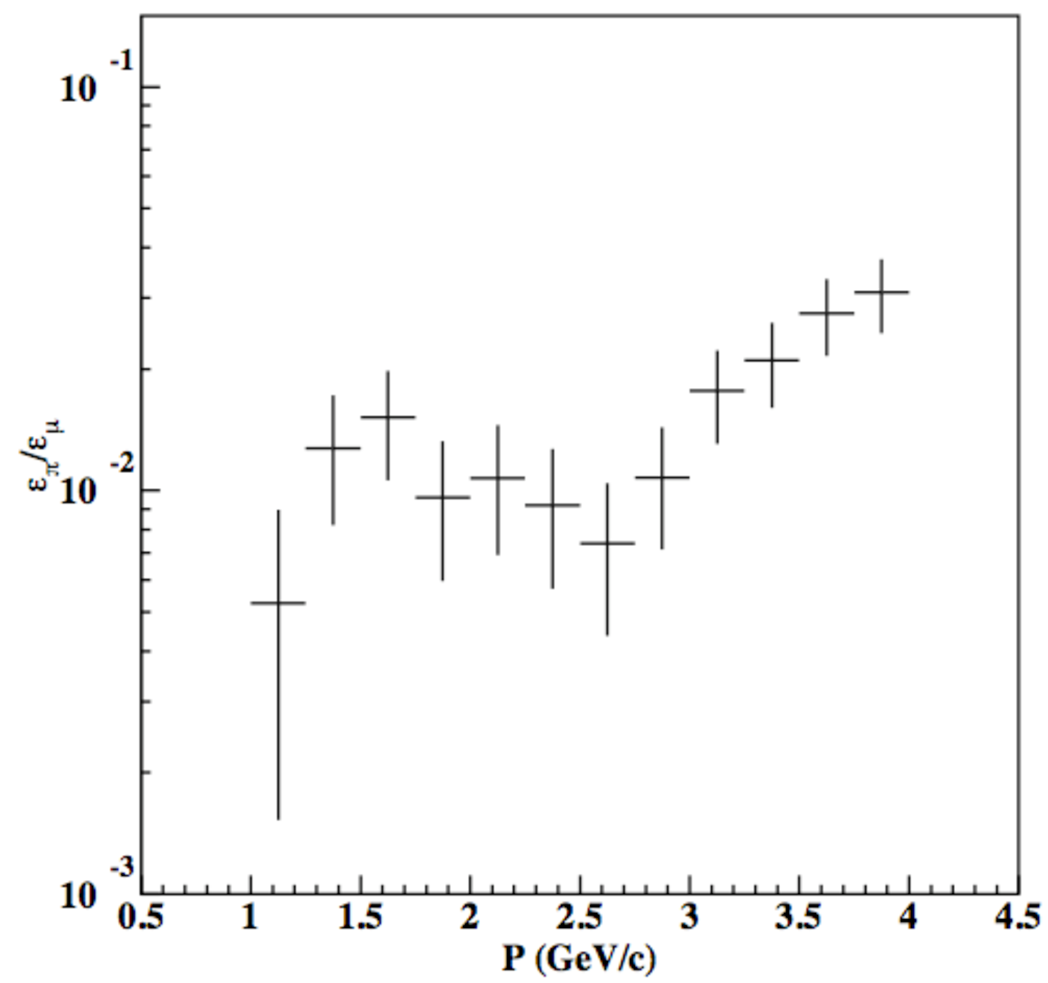
\includegraphics[scale=0.8]{muon/pmrej4.pdf}
\caption{\small{Pion-muon rejection factor as a function of the iron absorber thickness.}}\label{fig:pmrejp}
\end{figure*}

The simplest, most economical solution for the hodoscopes is to use layers of extruded scintillator strips with embedded wave-shifting fiber readout. The scintillator strips will be oriented horizontally. The light will be detected from both ends of the strip using multi-anode photomultipliers. With 5 cm vertical segmentation, a total of 144 readout channels are needed (9x16 channels multi-anode PMTs).  Signals from each channel will be sent to a TDC and to a FADC. The FADC information will be used to construct the muon trigger. The TDC information together with information from FADC will be used in offline analysis to measure the hit position along the strip. 
